\hypertarget{sec:solution}{%
\chapter{Lowering the initial hurdle to commence a web migration}\label{sec:solution}}

To address the problems identified in the state of the art of web migration that keep ISV, in particular SME-sized ISVs, from commencing a web migration, this chapter outlines the AWSM (Agile Web Migration for SMEs) \autocite{Heil2016AWSM} approach.
Based on the scenario introduced in \cref{sec:scenario}, an \emph{HCD\footnote{Human-Centered Design, cf.~http://www.designkit.org/} ideation process} comprising \emph{LFA\footnote{Logical Framework Approach, cf.~https://ec.europa.eu/europeaid/multimedia/publications/publications/manuals-tools/t101\_en.htm}-based problem analysis} provides a detailed understanding of the stakeholder-specific situation, concretises the factors of \emph{effort and risk} from the introduction, identifies three main research objectives and derives three corresponding solution opportunities which are described in the context of the AWSM Methodology and Platform.

\hypertarget{design-method-and-considerations}{%
\section{Design Method and Considerations}\label{design-method-and-considerations}}

This section describes the research methodology for designing the solution presented in \cref{sec:solution-overview}.
In \cref{sec:scenario} we introduced the main stakeholder role as SME-sized ISV with legacy, non-web, desktop application products and a large existing user base.

The research methodology aims at two objectives: to reach a better understanding of the stakeholder problem, i.e.~why are these ISVs hesitant to commence a web migration, what are the main concerns that create the organisational resistance, and to systematically devise a suitable approach addressing concrete solution opportunities derived from the problem analysis.

In addition to traditional requirements elicitation, methods from two methodologies have been employed: Human-Centered Design and Logical Framework Approach.
These will be briefly introduced and the application of methods described in the following.

\textbf{Human Centered Design (HCD)} is a paradigm for designing of solutions to problems with a focus on human needs and desires.
It has been defined with a technical scope for interactive systems and usability by ISO standard 9241-210 \autocite{ISO9241-210HCD}.
One of the main proponents and contributors of HCD is the design company IDEO\footnote{https://www.ideo.com/} that has assembled a systematic description of the methodology \autocite{HCD2015}.
The three-phase process comprises activities and artifacts that are used to get a deep understanding of problems from the human needs perspective, generate and select solution ideas and plan their implementation.
It is thus a tool for \emph{ideation}, that provides concrete guidelines and methods for conducting \emph{field research} in a design science context, which were applied for this thesis.

\textbf{Logical Framework Approach (LFA)} is a project planning and management methodology employed by the European Commission \autocite{Commission2004PCM} and other authorities.
It focuses on systematic \emph{problem and stakeholder analysis} and \emph{objective setting} in the analysis stage and is thus a tool for structuring observations gathered through HCD methods into concrete problem descriptions in this thesis.
In particular, \emph{LFA problem trees} allow to identify and represent cause-effect-relationships in the problem domain and are used to analyse the situation of the thesis' main stakeholder, ISVs with legacy software as characterised in \cref{sec:company-characteristics}.

\hypertarget{sec:research-process}{%
\subsection{Research Process}\label{sec:research-process}}

Figure \cref{fig:research-process} presents the four-phase research process combining methods from HCD and LFA, table \cref{tbl:research-methods} provides a mapping of these methods on the phases.

\begin{figure}
\hypertarget{fig:research-process}{%
\centering
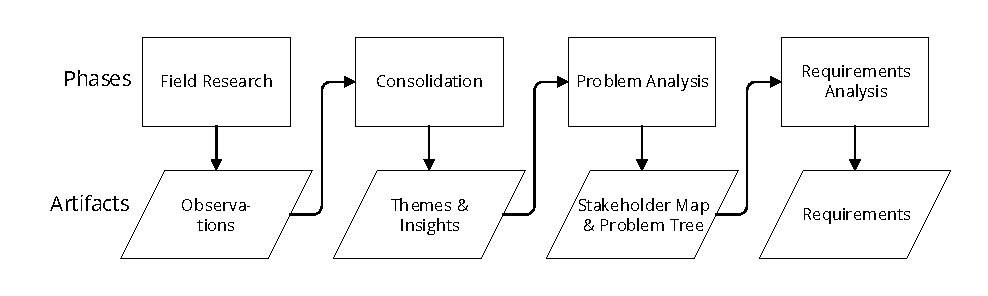
\includegraphics[width=0.99\textwidth]{../figures/20180115-DRF-Research-Process-Flow.pdf}
\caption{Research Process Flowchart}\label{fig:research-process}
}
\end{figure}

\hypertarget{tbl:research-methods}{}
\begin{longtable}[]{@{}ll@{}}
\caption{\label{tbl:research-methods}Methods used in Research phases}\tabularnewline
\toprule
\begin{minipage}[b]{0.28\columnwidth}\raggedright
Phase\strut
\end{minipage} & \begin{minipage}[b]{0.66\columnwidth}\raggedright
Methods\strut
\end{minipage}\tabularnewline
\midrule
\endfirsthead
\toprule
\begin{minipage}[b]{0.28\columnwidth}\raggedright
Phase\strut
\end{minipage} & \begin{minipage}[b]{0.66\columnwidth}\raggedright
Methods\strut
\end{minipage}\tabularnewline
\midrule
\endhead
\begin{minipage}[t]{0.28\columnwidth}\raggedright
Field Research\strut
\end{minipage} & \begin{minipage}[t]{0.66\columnwidth}\raggedright
HCD Recruiting Tools, Interviews, Extremes and Mainstream, Immersion, Guided Tour\strut
\end{minipage}\tabularnewline
\begin{minipage}[t]{0.28\columnwidth}\raggedright
Consolidation\strut
\end{minipage} & \begin{minipage}[t]{0.66\columnwidth}\raggedright
HCD Top Five, Find Themes, Create insight statements\strut
\end{minipage}\tabularnewline
\begin{minipage}[t]{0.28\columnwidth}\raggedright
Problem Analysis\strut
\end{minipage} & \begin{minipage}[t]{0.66\columnwidth}\raggedright
HCD Create Frameworks, LFA Stakeholder Analysis, LFA Problem Tree\strut
\end{minipage}\tabularnewline
\begin{minipage}[t]{0.28\columnwidth}\raggedright
Solution \& Research Design\strut
\end{minipage} & \begin{minipage}[t]{0.66\columnwidth}\raggedright
HCD How might we, Brainstorm, Get Visual, Prototyping, Feedback integration and iteration\strut
\end{minipage}\tabularnewline
\bottomrule
\end{longtable}

\textbf{Field research} was conducted at the headquarters of the SME-sized ISV medatixx (cf.~{[}@\#sec:company-characteristics{]}) to elicit observations as basis for systematic problem analysis.
Several methods from HCD's Inspire phase were employed: \emph{Recruiting Tools} helped identify people to talk to, including senior management (``Leiter Softwareproduktion'' - Head of Development), middle management (``Abteilungsleiter Softwareproduktion'' - Head of Software Development Department) and staff (software engineers, software testers, scrum masters, product owners, DevOps, maintenance) and, following the \emph{Extremes and Mainstream} method including both proponents and opponents of web migration.
A \emph{Guided Tour} was taken to get to know the different development teams, organizational structures and work environment.
The observations were elicited using \emph{Interviews} in groups and single and using in-context \emph{Immersion}.
This method was particularly fruitful, comprising a one-week integration in a scrum team, actively participating in development activities and meetings.
This provided a good understanding of the daily development practice, expertise level of staff and a solid trust basis for interviews and subsequent feedback cycles.
More than 50 observations of the field research phase were captured and organised using Trello\footnote{https://trello.com/} cards.

\textbf{Consolidation} was used to abstract from the concrete observations into themes that capture relevant and recurring problem patterns.
This was supported by HCD's Ideation phase methods.
\emph{Find Themes} in combination with the collaborative filtering proposed in the \emph{Top Five} method was used to cluster the observations and identify the most relevant problem areas.
\emph{Insight statements} were created for the themes from observations.
The themes and insights were captured on post-its to provide the input for problem analysis.

\textbf{Problem Analysis} considered the relationships between the insights and themes to create a systematic view of the problem domain.
According to HCD's \emph{Create Frameworks} method an initial relational map was created.
LFA \emph{stakeholder analysis} was conducted to capture the stakeholder map which systematically describes characteristics and intensions of the involved roles.
The problem hierarchy was identified bottom-up from the insights and themes and their cause-effect relationships and represented as a LFA \emph{problem tree}.
The results of the problem analysis phase were iteratively improved through a feedback loop with the ISV and are outlined in \cref{sec:problem-analysis-results}.

\textbf{Solution \& Research Design} transformed the problem analysis results into a solution design representing a set of research questions.
A sub-tree of relevant problems according to the scope of this thesis \cref{sec:scope} was selected and \emph{How Might We} questions were formulated to drive ideation of opportunities (solution ideas) in the collaborative \emph{brainstorm} session.
To communicate the solution ideas, \emph{visual} representations (cf.~paper prototypes in \todo{TODO:REF\_ANNOTATION\_CHAPTER)} and software \emph{prototypes} were created.
\emph{Feedback Integration and Iteration} was used to improve the opportunities through stakeholder feedback gathered in a presentation and discussion session at the ISVs headquarters and continued throughout the entire research project.
Eventually, partial research questions were derived which define the solution parts on a coarse-grain level.
The resulting solution \& research design is described in \cref{sec:solution-overview}.

\hypertarget{sec:problem-analysis-results}{%
\subsection{Problem Analysis Results}\label{sec:problem-analysis-results}}

As part of the problem analysis, we identified stakeholders and their characteristics in terms of their interests and how they are affected by a web migration, their capacity and motivation, and possibilities to address and engage them.
Table \cref{tbl:stakeholders} shows the results.
The ISV stakeholder is further detailed in two distinct roles: \emph{Management} and \emph{Software Engineers}.
Management is responsible for the decision to migrate and is aware of the risks and thus must be addressed through risk management and communication of benefits.
Software Engineers are the group of potential actors of web migration, they define the requirements for migration activities through their expertise and development processes and tailored methods need to be provided that reduce migration workload.
We will use the term \emph{Migration Engineer} to refer to a Software Engineer who is performing web migration activities.
Migration Engineers are to be considered a sub-class of Software Engineers, i.e.~all super-class characteristics apply.
Two customer stakeholders exist: the \emph{doctor's offices} are the direct customer of the PMS ISV whereas \emph{patients} are the customers of the customers and benefit most from innovative features and improved usability and interactivity.
Furthermore, \emph{competitors} are affected by the affects on market share of increased competitiveness of the ISV through web migration and \emph{companies with similar situation}, i.e.~other ISVs with non-web legacy systems and large user bases can benefit from the dissemination of results to apply to their situation.

\hypertarget{tbl:stakeholders}{}
\begin{longtable}[]{@{}llll@{}}
\caption{\label{tbl:stakeholders}Stakeholder Map}\tabularnewline
\toprule
\begin{minipage}[b]{0.16\columnwidth}\raggedright
Stakeholder\strut
\end{minipage} & \begin{minipage}[b]{0.24\columnwidth}\raggedright
Interest/how affected\strut
\end{minipage} & \begin{minipage}[b]{0.24\columnwidth}\raggedright
Capacity \& Motivation\strut
\end{minipage} & \begin{minipage}[b]{0.24\columnwidth}\raggedright
Possible Actions to Address Stakeholders\strut
\end{minipage}\tabularnewline
\midrule
\endfirsthead
\toprule
\begin{minipage}[b]{0.16\columnwidth}\raggedright
Stakeholder\strut
\end{minipage} & \begin{minipage}[b]{0.24\columnwidth}\raggedright
Interest/how affected\strut
\end{minipage} & \begin{minipage}[b]{0.24\columnwidth}\raggedright
Capacity \& Motivation\strut
\end{minipage} & \begin{minipage}[b]{0.24\columnwidth}\raggedright
Possible Actions to Address Stakeholders\strut
\end{minipage}\tabularnewline
\midrule
\endhead
\begin{minipage}[t]{0.16\columnwidth}\raggedright
Management\strut
\end{minipage} & \begin{minipage}[t]{0.24\columnwidth}\raggedright
- higher sales- reduced costs for software distribution and maintenance- increased risk and workload through migration\strut
\end{minipage} & \begin{minipage}[t]{0.24\columnwidth}\raggedright
- decision taker role- higher competitiveness due to improved product portfolio and reduced effort\strut
\end{minipage} & \begin{minipage}[t]{0.24\columnwidth}\raggedright
- risk management- communicate benefits through prototypes\strut
\end{minipage}\tabularnewline
\begin{minipage}[t]{0.16\columnwidth}\raggedright
Software Engineers (Migration Engineers)\strut
\end{minipage} & \begin{minipage}[t]{0.24\columnwidth}\raggedright
- new knowledge- increased workload through migration\strut
\end{minipage} & \begin{minipage}[t]{0.24\columnwidth}\raggedright
- key role, defining available expertise and requirements for migration activities- limited motivation improvement of product and lower effort for updates and maintenance\strut
\end{minipage} & \begin{minipage}[t]{0.24\columnwidth}\raggedright
- presentation of technology demonstrators etc.- reduce workload through tailored and integrated migration methods and tools\strut
\end{minipage}\tabularnewline
\begin{minipage}[t]{0.16\columnwidth}\raggedright
Doctor's Offices\strut
\end{minipage} & \begin{minipage}[t]{0.24\columnwidth}\raggedright
- innovative features \& improved usability- changes in existing work patterns- training effort- new hardware- security and data privacy\strut
\end{minipage} & \begin{minipage}[t]{0.24\columnwidth}\raggedright
- customers- almost no intrinsic motivation\strut
\end{minipage} & \begin{minipage}[t]{0.24\columnwidth}\raggedright
- user training\strut
\end{minipage}\tabularnewline
\begin{minipage}[t]{0.16\columnwidth}\raggedright
Patients\strut
\end{minipage} & \begin{minipage}[t]{0.24\columnwidth}\raggedright
- innovative features \& improved usability- more interactivity\strut
\end{minipage} & \begin{minipage}[t]{0.24\columnwidth}\raggedright
- customers of customers\strut
\end{minipage} & \begin{minipage}[t]{0.24\columnwidth}\raggedright
- information about new features\strut
\end{minipage}\tabularnewline
\begin{minipage}[t]{0.16\columnwidth}\raggedright
Competitors\strut
\end{minipage} & \begin{minipage}[t]{0.24\columnwidth}\raggedright
- idea transfer to own products - competitive disadvantage\strut
\end{minipage} & \begin{minipage}[t]{0.24\columnwidth}\raggedright
- market share\strut
\end{minipage} & \begin{minipage}[t]{0.24\columnwidth}\raggedright
N/A\strut
\end{minipage}\tabularnewline
\begin{minipage}[t]{0.16\columnwidth}\raggedright
Companies with similar situation\strut
\end{minipage} & \begin{minipage}[t]{0.24\columnwidth}\raggedright
- solution\strut
\end{minipage} & \begin{minipage}[t]{0.24\columnwidth}\raggedright
- improved situation\strut
\end{minipage} & \begin{minipage}[t]{0.24\columnwidth}\raggedright
- dissemination of Results\strut
\end{minipage}\tabularnewline
\bottomrule
\end{longtable}

This knowledge about the stakeholders together with themes and insights from the consolidation phase needed into the analysis of problems and problem relationships.
The problem hierarchy is presented in \cref{fig:problem-tree}.
While it was created bottom-up, starting with insights, we will briefly outline the problem tree top-down for easier understanding.
The arrows in the LFA tree indicate cause-effect relationships, with effects represented in direction of the arrows and causes in the opposite direction.

The root-level problem is the competitiveness of the ISV (effects of this problem such as losing market shares to competition are not shown for brevity).
This jeopardised by both the consequences of maintaining a legacy system and technical debt (cf.~\cref{sec:situation}) leading to \emph{overloading} of staff and the \emph{hesitation to commence web migrate} due to \emph{doubts about feasibility and desirability} (cf.~also to resistance from organization in \autocite{Khadka2014ProfessionalsModernization,Sneed2010ReMiP}).
The legacy-characteristic causes of overloading, such as low maintainability due to \emph{side-effects}, \emph{technological deprecation}, \emph{multi-platform environment} and \emph{limited time \& resources} are pushing factors in favour of a web migration.
On the other hand, risk and effort of a web migration constitute \emph{doubts about feasibility and desirability}.
In particular, \emph{limited time and resources} for conducting the migration, \emph{unknown plausibility of a web-based version}, difficult \emph{integration into ongoing development}, and a \emph{lack of knowledge of methods and technologies} regarding migration and staff with \emph{web engineering expertise} feed into feasibility doubts.
Likewise, \emph{lack of a deeper understanding of potential benefits}, the \emph{risk of losing poorly documented knowledge} and \emph{potential impact on existing customers} through abrupt changes form doubts about desirability of web migration.
The root causes on the lowest level of the problem tree are \emph{architectural degradation} of the legacy systems, \emph{missing documentation and experience of legacy code}, a \emph{strict release cycle regime} due to regulatory and contractual constraints, lack of \emph{staff with web engineering expertise} and a large existing \emph{customer base whose workflows are oriented on the user interaction of the software products}.
The latter three problems are situational problems that impose constraints on potential solutions as represented in requirements C4 Agile, C3 Exp and C2 Reuse.

\begin{figure}
\hypertarget{fig:problem-tree}{%
\centering
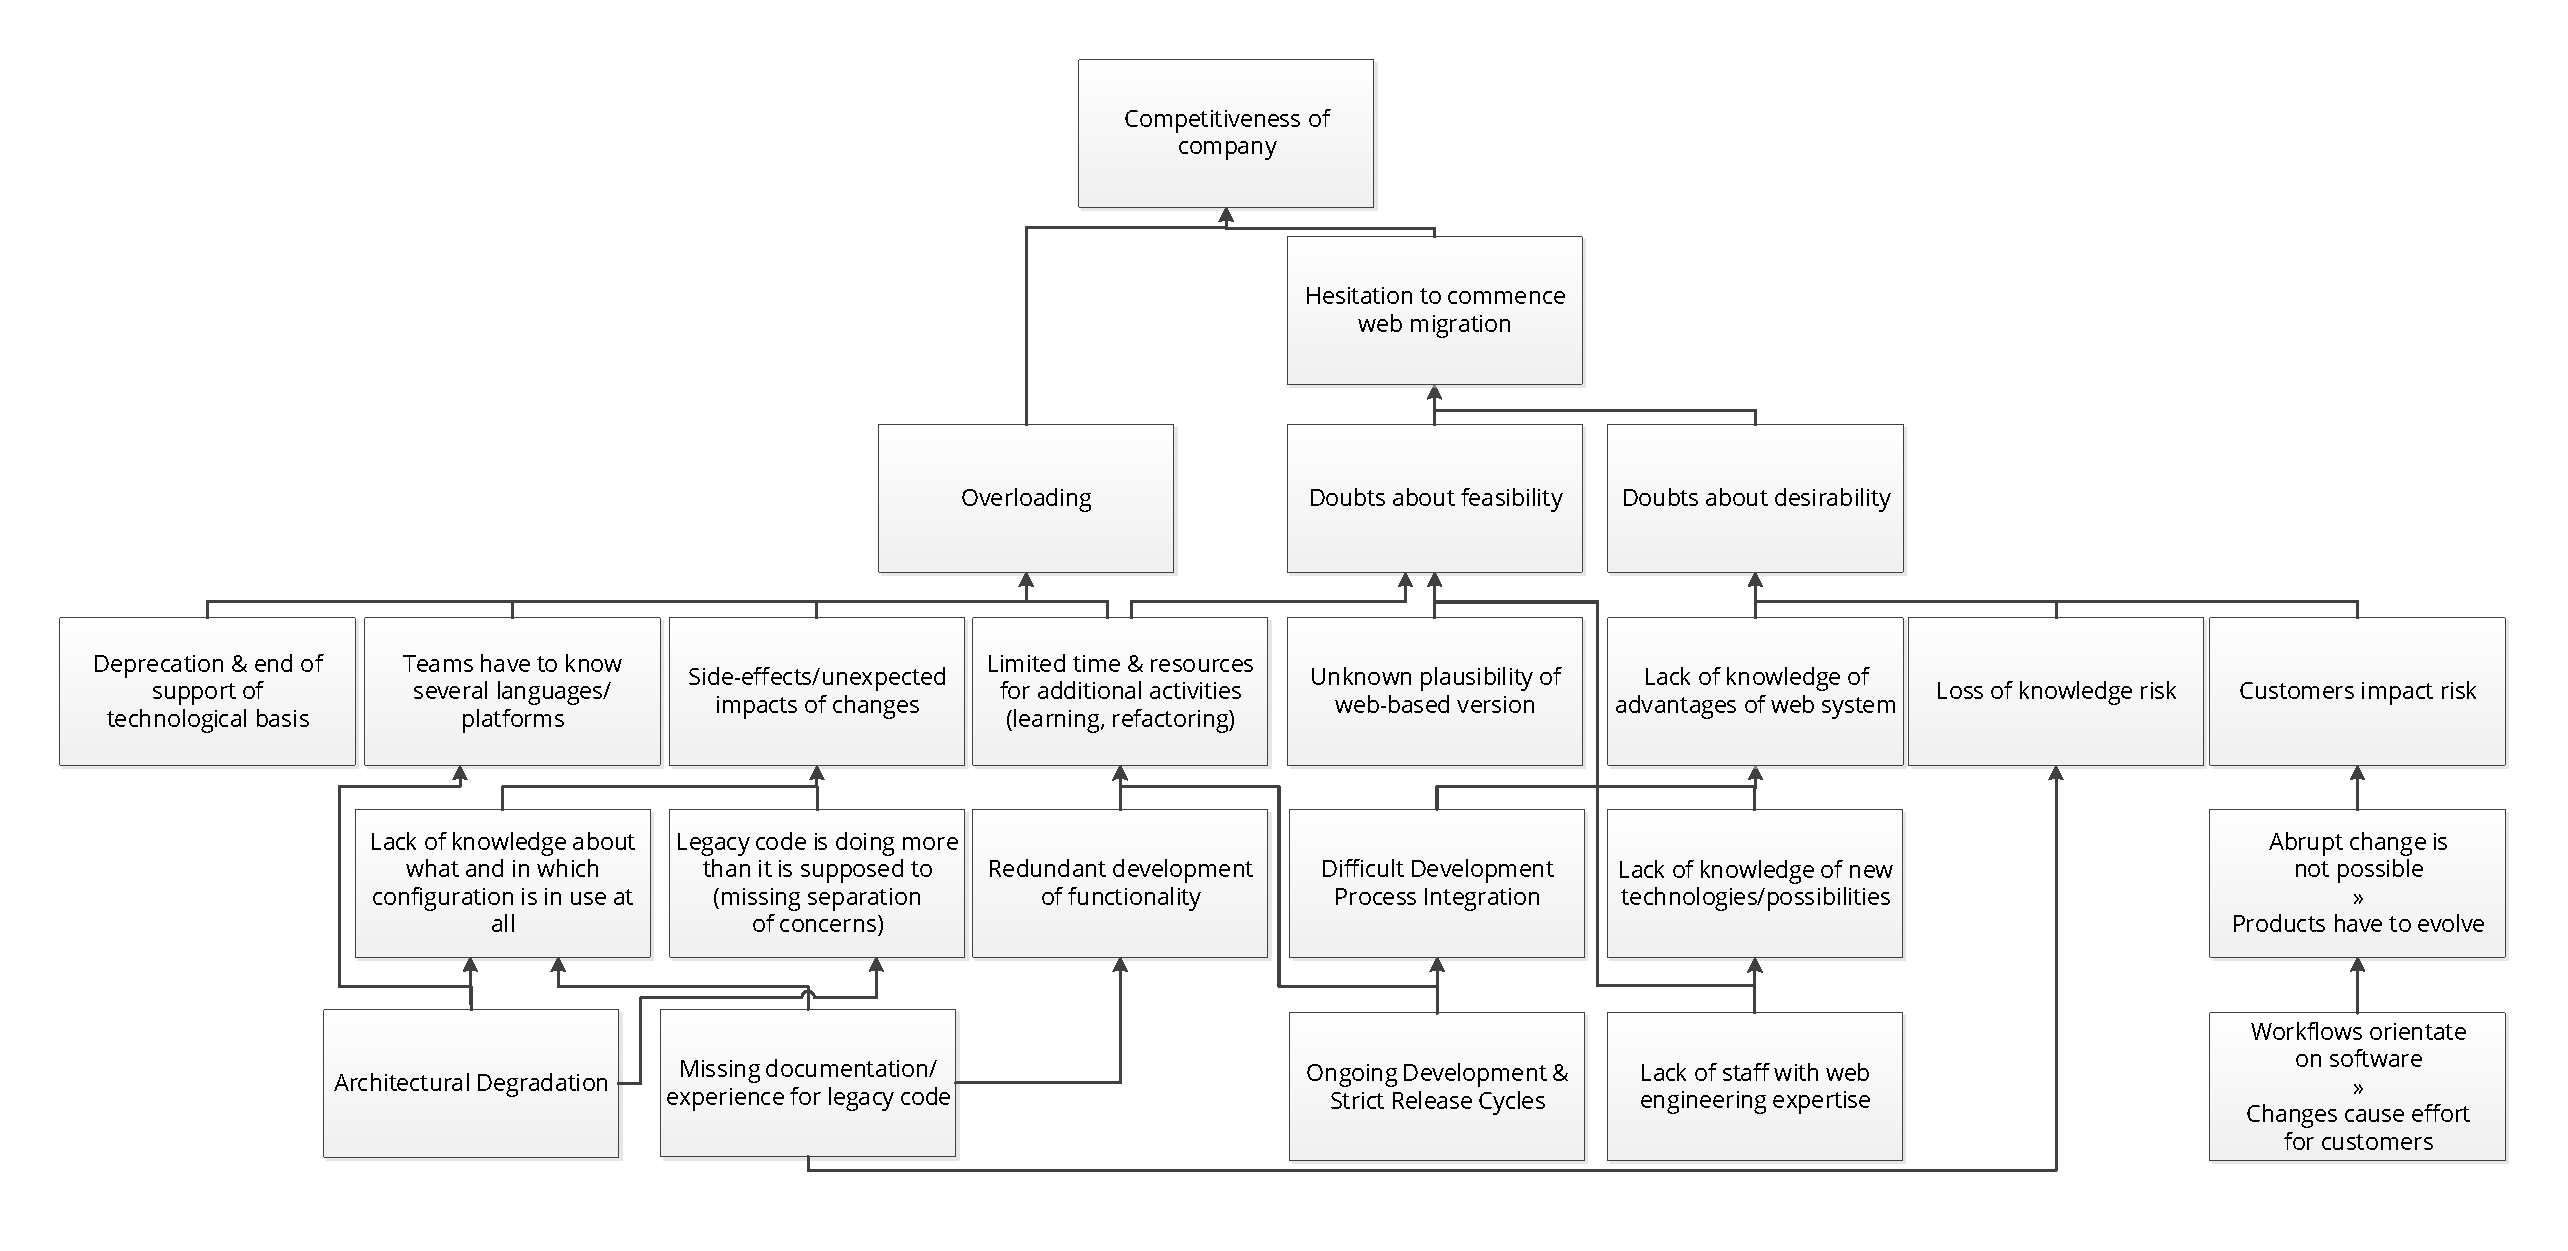
\includegraphics[width=0.99\textwidth]{../figures/20180115-DRF-Problem-Tree.pdf}
\caption{Hierarchical Representation of Problem Domain as LFA Problem Tree}\label{fig:problem-tree}
}
\end{figure}

\hypertarget{solution-research-design}{%
\subsection{Solution \& Research Design}\label{solution-research-design}}

The main research question of this thesis, RQ1, directly corresponds to the \emph{hesitation to commence web migration} problem and its corresponding sub-tree in \cref{fig:problem-tree}.
The detailed problem analysis shows that the \emph{effort and risk} factors described in literature (cf.~\cref{sec:problem}) that make companies hesitant to commence a web migration can be concretized into the problems of \emph{doubts about feasibility} and \emph{doubts about desirability} for ISVs with non-web legacy systems and large existing user bases.

Through reformulation using the How-Might-We method of HCD, the intial research question RQ 1

\begin{quote}
\emph{How might we support companies to commence web migration?}
\end{quote}

translates into

\begin{quote}
How might we address IVS's doubts about feasibility and desirability?
\end{quote}

which defines the solution scope.
Aligned with the problem tree, this question is further broken down into the three questions HMW1 - HMW3 in \cref{tbl:hmw}.

\hypertarget{tbl:hmw}{}
\begin{longtable}[]{@{}ll@{}}
\caption{\label{tbl:hmw}How Might We Questions for Ideation of Research Objectives}\tabularnewline
\toprule
\begin{minipage}[b]{0.06\columnwidth}\raggedright
ID\strut
\end{minipage} & \begin{minipage}[b]{0.88\columnwidth}\raggedright
Question\strut
\end{minipage}\tabularnewline
\midrule
\endfirsthead
\toprule
\begin{minipage}[b]{0.06\columnwidth}\raggedright
ID\strut
\end{minipage} & \begin{minipage}[b]{0.88\columnwidth}\raggedright
Question\strut
\end{minipage}\tabularnewline
\midrule
\endhead
\begin{minipage}[t]{0.06\columnwidth}\raggedright
HMW1\strut
\end{minipage} & \begin{minipage}[t]{0.88\columnwidth}\raggedright
How might reduce the risk of loss of knowledge through web migration?\strut
\end{minipage}\tabularnewline
\begin{minipage}[t]{0.06\columnwidth}\raggedright
HMW2\strut
\end{minipage} & \begin{minipage}[t]{0.88\columnwidth}\raggedright
How might we demonstrate feasibility and advantages of a web-based version of the legacy system?\strut
\end{minipage}\tabularnewline
\begin{minipage}[t]{0.06\columnwidth}\raggedright
HMW3\strut
\end{minipage} & \begin{minipage}[t]{0.88\columnwidth}\raggedright
How might we reduce the risk of customers impact through web migration?\strut
\end{minipage}\tabularnewline
\begin{minipage}[t]{0.06\columnwidth}\raggedright
HMW4\strut
\end{minipage} & \begin{minipage}[t]{0.88\columnwidth}\raggedright
How might we address HMW1, HMW2 and HMW3 with limited resources and lack of web engineering expertise?\strut
\end{minipage}\tabularnewline
\bottomrule
\end{longtable}

These questions address the problem sub-trees of feasibility and desirability doubts from the perspective of \emph{functional requirements} in classical requirements engineering.
To represent the situation and constraints of the ISV, HMW4 represents the \emph{non-functional requirements} perspective.

Based on RQ1 and HMW4, the research objective of this thesis is:

\textbf{Research Objective RO1}

\begin{quote}
To provide methods, models and tools that support ISVs with limited resources and lack of web engineering expertise to commence a web migration.
\end{quote}

To achieve this objective, three specific research objectives were identified from RQ2 - RQ4 employing HCD-based opportunity ideation described in \cref{sec:research-process}.
These objectives are:

\textbf{Research Objective RO2}

\begin{quote}
To provide a reverse engineering method that allows to identify and manage existing knowledge in legacy source code with limited resources and lack of web engineering expertise.
\end{quote}

\textbf{Research Objective RO3}

\begin{quote}
To provide a risk management method that demonstrates desirability and feasibility of a potential web-based version of the legacy system with limited resources and lack of web engineering expertise.
\end{quote}

\textbf{Research Objective RO4}

\begin{quote}
To provide an HCI method to control the impact of web migration on customers with limited resources and lack of web engineering expertise.
\end{quote}

These research objectives define the solution specified in the following section.

\begin{figure}
\hypertarget{fig:objectives}{%
\centering
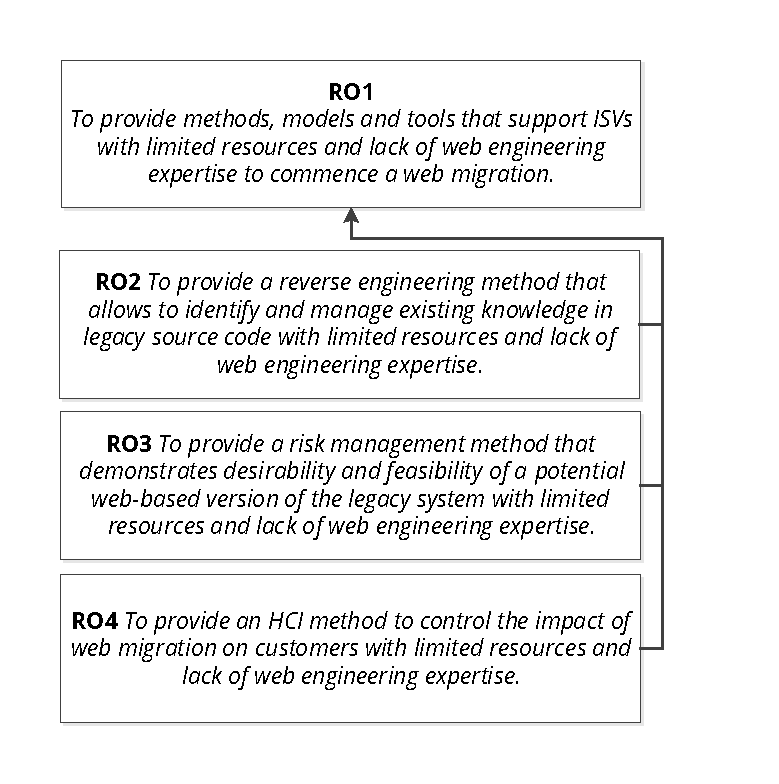
\includegraphics[width=0.99\textwidth]{../figures/objectives.pdf}
\caption{Research Objectives}\label{fig:objectives}
}
\end{figure}

\hypertarget{sec:solution-overview}{%
\section{Agile Web Migration for SMEs}\label{sec:solution-overview}}

Our solution to address RO1 to RO4 is \emph{AWSM (Agile Web Migration for SMEs)} \autocite{Heil2016AWSM}.
Figure \cref{fig:solution} shows the architecture of AWSM.
It consists of the \emph{AWSM Methodology} which is supported by the \emph{AWSM Platform} and leverages three solution components corresponding to research objectives RO2, RO3 and RO4: the AWSM reverse engineering method, the AWSM risk management method and the AWSM customer impact control method.
AWSM is structured according to the constructive elements of software engineering for quality ensurance \autocite{Wallmueller2001SoftwareQuality} into Principles, Formalisms, Methods and Tools.
The AWSM Methodology describes principles formalisms and methods.
Corresponding support Tools constitute the AWSM Platform.
\emph{Principles} are at the foundation of AWSM and drive design decisions of the AWSM Methodology and Platform in addition to the identified requirements.
\emph{Formalisms} are the conceptual basis for the methods and tools.
They specify the underlying mathematical model and semantics for knowledge in legacy source code and the definition and algorithm for measuring similarity between original and migrated user interfaces.

\begin{figure}
\hypertarget{fig:solution}{%
\centering
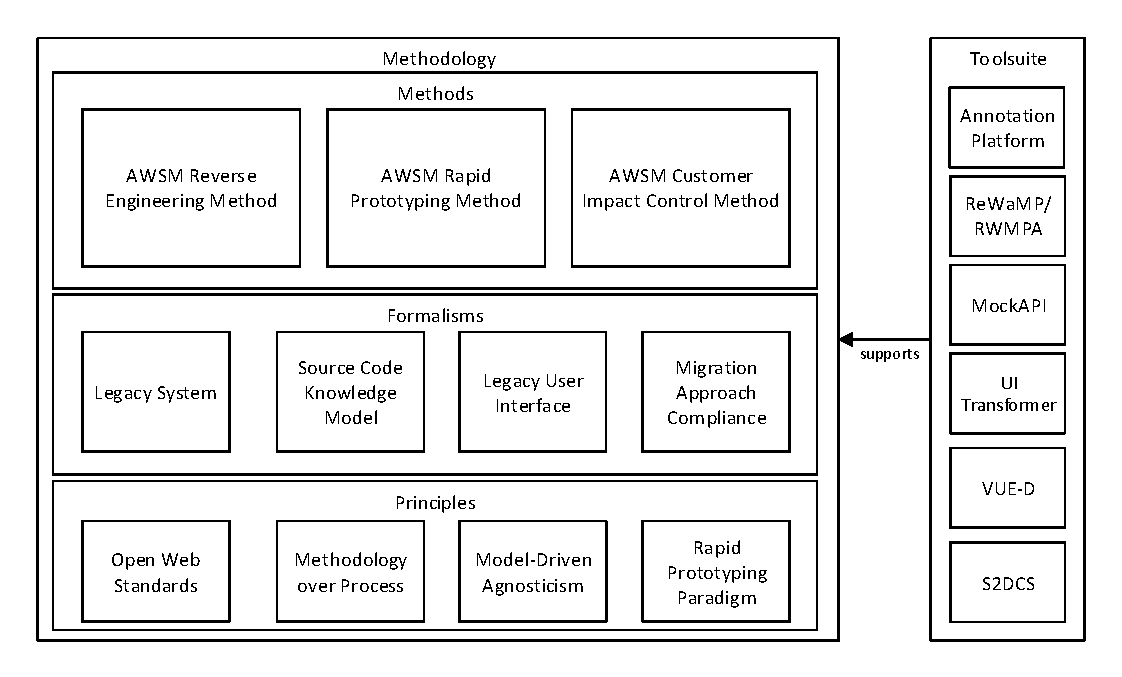
\includegraphics[width=0.99\textwidth]{../figures/solution.pdf}
\caption{AWSM Overview}\label{fig:solution}
}
\end{figure}

\todo{TODO:add RWMPA}, UI Generator\textgreater UI Transformer, ReWaMP

\hypertarget{awsm-methodology}{%
\section{AWSM Methodology}\label{awsm-methodology}}

According to RO1, AWSM addresses shortcomings of existing web migration approaches in initial phases of migration projects.
Similar to SMART \autocite{Lewis2008SMART,Lewis2005SMART}, it does not impose a specific migration process.
Thus, the AWSM Methodology focuses on principles, formalisms and methods for web migration initiation and integration with existing comprehensive migration methods.
It can be combined with incremental reengineering and transformation processes.
AWSM addresses a package-oriented \autocite{Brodie1995Migrating} feature-driven \autocite{Menychtas2014ARTISTJournal} incremental process model.

\hypertarget{principles}{%
\subsection{Principles}\label{principles}}

The following principles are the form the basis for the AWSM Methodology and Platform and, in addition to the requirements, drive the design decisions.

\textbf{P1 Open Web Standards} The use of standards is widely accepted in software engineering and web engineering.
This principle advocates using and extending open web standards, in particular W3C specifications and OMG standards, to allow interoperability with existing methods and tools and provide contributions that can easily be used and enhanced by future research (cf.~OpenStand Principles\footnote{https://open-stand.org/about-us/principles/}).
This especially applies to underlying data models, provided interfaces and technologies used.

\textbf{P2 Methodology over Process} As shown in \cref{sec:approaches}, there is a wide range of existing web migration approaches with corresponding process models.
However, these approaches are lacking in the aspects important for web migration initiation for ISVs with limited resources and lack of web engineering expertise.
Thus AWSM aims at providing a methodology that addresses these shortcomings with formalisms, methods and tools.
This principle advocates an openness for existing web migration reengineering and transformation process models to prefer re-use over re-definition of a new web migration process model.
Therefore, AWSM methods need to define mappings for extension of the most relevant web migration approaches such as REMICS, ARTIST or UWA/UWAT+.

\textbf{P3 Model-Driven Agnosticism} The current web migration landscape is divided on the use of Model-Driven Engineering (MDE).
In \cref{sec:approaches} half of the approaches employ MDE in some form, half of the approaches does not.
Similarly MDE practices are employed in varying degrees in forward web engineering \autocite{Moreno2008MDWE}.
Thus this principle advocates an openness to different degrees of Model-Driven and Non-Model-Driven approaches for the core methods of the methodology.
In particular reverse engineering, which forms the basis of reengineering and transformation, should be laid out agnostic but adaptable to concrete Model-Driven or Non-Model-Driven methods to allow interoperability with a wide range of existing web migration approaches.

\textbf{P4 Rapid Prototyping Paradigm} Prototyping is an established means of improving quality in forward software engineering \autocite{Wallmueller2001SoftwareQuality}.
The rapid prototyping paradigm \autocite{Gordon1995RapidPrototyping} with its dedicated focus on quick and cheap creation of tangible means of communication of envisioned software for all involved stakeholders \autocite{Alavi1984} has become particularly popular in the context of Agile Development \autocite{Abrahamsson2002Agile} and Human-Centered Design \autocite{HCD2015}.
Thus this principle advocates applying the rapid prototyping paradigm to the web migration domain by favouring the creation of concrete, tangible means of communication to demonstrate feasibility and desirability of a web-based version of the migrated legacy system over theoretical and general argumentation and narrowly focused technical feasibility studies.

\hypertarget{sec:formalisms}{%
\subsection{Formalisms}\label{sec:formalisms}}

The following formalisms form the theoretical basis of the AWSM methods.
They define basic conceptual models independent of their concrete implementation in the AWSM platform.
The conceptual architecture of the AWSM platform is discussed in \cref{sec:platform}.
Following principle P1, the formalisms are based on the OMG's Knowledge Discovery Meta-Model specification, which is designed in a partitioned way to allow adopters to effectively use only parts ``necessary for their activities'' \autocite{OMG2016KDM}.
For brevity, when referring to KDM in the following description of formalisms, these references are to be considered as reference to KDM version 1.4 of September 2016 \autocite{OMG2016KDM}.

\textbf{Legacy System}

The legacy system is the basis for any web migration and the central object of investigation of this thesis, serving as the starting point for the three AWSM methods.
KDM \autocite{OMG2016KDM} provides a comprehensive metamodel for describing legacy systems.
This section describes the conceptual model of a legacy system based on a subset of KDM concepts which provides the common foundation for the understanding of legacy systems in the context of the AWSM methodology.
In particular, the \emph{inventory model} of the KDM \emph{source package}, the \emph{platform package} and the \emph{UI package} are relevant for AWSM.
A legacy system \(\mathfrak{L}\) is a tuple

\begin{equation}\mathfrak{L} = (B, Dep, \underline D,  E, D, U)\label{eq:legacy-system}\end{equation}

\(B\) is the legacy codebase consisting of a set of source code files (SourceFile in KDM), configuration files (KDM \emph{ConfigFile}) and other textual documents (KDM \emph{Document}).
\(Dep\) are the dependencies of the legacy system (KDM: \emph{LinkableFile}), in particular third-party libraries (KDM: \emph{LibraryFile}).
The dependency matrix \(\underline D: \{1,\ldots, |B|\} \times \{1,\ldots, |Dep|\} \mapsto [0,1]\) is a binary matrix with \(\underline D_{i,j} = 1 \Longleftrightarrow f_i \in B\) depends on \(dep_j \in Dep\), else \(\underline D_{i,j} = 0\).
\(E\) are the executables (KDM \emph{ExecutableFile}) of the legacy system.
In some scenarios \(B\) or \(E\) can be \(B=E=\emptyset\) \todo{TODO:REF}, however, as described in \cref{sec:scenario-code}, we assume availability of source code and executables in this thesis.
\(D\) represents the persistent data of the legacy system such as databases (KDM: \emph{DataManager}), storage files (KDM: \emph{FileResource}), XML or JSON files (KDM: \emph{DataFile}).
\(U\) is the set of resources that form the user interface (KDM: \emph{UIModel}) of the legacy system, consisting of container resources (KDM: \emph{UIResource}) like screens.
The elements of \(U\) are not identical to their formal representation in \(B\) (e.g.~XAML files, MFC recource files), but they are resulting from it and part of the executables in \(E\) from where their visual (i.e.~pixel-based) representation can be retrieved.
The legacy user interface is described in more detail in \cref{sec:ui-formalism}.

This conceptual model describes a legacy system in terms of its \emph{software artifacts} \autocite{OMG2016KDM}, i.e.~of physical resources that are available as inputs for analysis and transformation activities described in the methods of the AWSM methodology.
In contrast, the following source code knowledge model formalism describes the relevant \emph{software assets} \autocite{OMG2016KDM} that are represented through the artifacts but not necessarily in existing explicit forms.

\textbf{Source Code knowledge model}

The source code knowledge model (SCKM) is at the core of the AWSM reverse engineering method.
As argued in the introduction, legacy systems contain valuable \emph{knowledge from problem and solution domain} \autocite{Marcus2004ProblemLocation} that must be preserved throughout migration.
Loss of knowledge is a risk (cf.~C1 Risk and HMW1) that needs to be addressed to assist web migration initiation (cf.~RO2).
Knowledge in legacy code bases is implicit: similar to \emph{tacit knowledge} in organizations which is
not expressed explicitly but guides human behaviour \autocite{Nonaka2008TacitKnowledge}, the knowledge legacy systems is not explicitly documented but governs how they operate.
Codification
\autocite{Hansen1999KnowledgeManagement} is required to make it explicit, which is achieved through \emph{reverse engineering}.
The knowledge reverse engineered from the legacy source code through \emph{redocumentation} and \emph{design recovery} needs to be represented at different levels of abstraction \autocite{Chikofsky1990ReverseEngineering} and stored in a knowledgebase to feed into subsequent reengineering or transformation.
OMG's ADM provides a basic model for legacy source code knowledge above procedure level in the KDM specification as described in \cref{sec:adm}.
Thus it is used as basis for the SCKM.
However, KDM is focused on redocumentation knowledge, i.e.~equivalent representations of knowledge within the same abstraction level, the implementation level \autocite{Chikofsky1990ReverseEngineering}, allowing to describe the structure of the legacy codebase in terms of modules, classes, methods, files.
In particular, KDM often assumes knowledge to reside in dedicated files - data in data files, configuration in configuration files etc.
- whereas knowledge often appears mixed, due to missing separation of concerns in legacy systems \autocite{Rodriguez-Echeverria2010MIGRARIA}, within source code.
The SCKM extends KDM towards representation of design recovery knowledge, i.e.~knowledge on higher levels of abstraction while maintaining the connection to its occurrence in structural parts of the source code.

Migration aims at retaining functionality of legacy systems in new environments \autocite{Bisbal1999LegacyInformationSystems}, with functionality referring to domain knowledge and business logic \autocite{Wagner2014}.
Thus, there are two basic types of knowledge in legacy source code: Features and domain knowledge.
\emph{Features} describe functionality of the legacy system (What) \autocite{SWEBOK2014,Rubin2013FeatureLocation,Rajlich2002Concepts} and can be represented as user stories, scenarios, use cases (KDM: \emph{ScenarioUnit}) etc..
\emph{Domain knowledge} is the knowledge supporting the implementation of features, describing parts of the problem and solution domain of the legacy system (How) \autocite{Marcus2004ProblemLocation,Rajlich2002Concepts}.
Typically, three categories corresponding to a classical three-tier-architecture are considered in program decomposition: \emph{presentation} (KDM \emph{UI domain}), \emph{application logic} (KDM \emph{ConceptualFlow}) and \emph{persistence} (KDM \emph{data domain}) \autocite{Canfora2000Decomposing}.
Presentation comprises information about the user interface layout and the user interaction handling.
Persistence defines knowledge about data models, data flow, caching etc.
The SCKM extends the three basic categories allowing a more detailed distinction of domain knowledge in source code.
In particular, \emph{business processes} and \emph{business rules} (KDM \emph{RuleUnit}) \autocite{Aversano2001,Sneed2010SoftwareMigration,Wagner2014Fundamentals,Ulrich2011} are crucial problem domain knowledge.
Solution domain knowledge comprises \emph{algorithms} (KDM: \emph{BehaviorUnit}), \emph{configuration} (KDM: \emph{ConfigFile}) and \emph{deployment} (KDM: \emph{Deployment}).
Note that both business processes and algorithms describe processes in the source code, but business processes are processes that exist in the problem domain whereas algorithms are solution domain processes.
Furthermore, legacy systems can contain \emph{explanatory} natural-language knowledge embedded in the code as comments (KDM: \emph{CommentUnit}).
A similar distinction can be found in the taxonomy of legacy artifacts in ARTIST
\autocite{ARTIST2013Taxonomy}.

While KDM relates knowledge to physical artifacts like files and structural elements like classes, the SCKM considers knowledge to be an independent software asset that can be related to arbitrary parts of \(\mathfrak{L}\).
These knowledge types can be represented by a variety of representations like UML class diagrams, BPMN diagrams, flow charts, SBVR\footnote{https://www.omg.org/spec/SBVR/} rules, other forms of models (KDM: \emph{Model}), informal or semi-formal natural language texts etc., depending on the intended use (cf.~principles P2 and P3) and can even have no representation (\(r=0\)) since knowing the type of a certain piece of \(\mathfrak{L}\) is already knowledge.

Thus, an instance of knowledge \(k\) in the legacy system \(\mathfrak{L}\) is a tuple

\begin{equation}k = (t, r)\label{eq:knowledge}\end{equation}

of type \(t \in T\) and a representation \(r\).
\begin{equation}T = \{\textrm{feature}, \textrm{presentation}, \textrm{persistence}, \textrm{business rule}, \textrm{business process}, \textrm{algorithm}, \textrm{configuration}, \textrm{deployment}, \textrm{explanatory}\}\label{eq:knowledge-types}\end{equation}

As this knowledge is implicitly represented and distributed (e.g.~partial classes) in the source code, it is crucial to codify the connection between the knowledge representation and its occurrences in the source \autocite{Rajlich2002Concepts}, in particular considering the importance of decomposability for migration \autocite{Lucia2008,Canfora2000Decomposing}.
Based on the conceptual model of KDM, the location \(l\) can be specified as a reference (KDM: \emph{SourceRef}) to a specific segment of code \(s\) (KDM: \emph{SourceRegion}) within a physical source code artifact \(f \in B\) (KDM: \emph{SourceFile}) of the legacy codebase.
The source file content is interpreted as linear stream of characters, allowing to define a segment in terms of inclusive start \(\alpha\) and end \(\omega\) position in that stream:

\begin{equation}l = (s,f)\label{eq:location}\end{equation}

\begin{equation}s=(\alpha, \omega) \textrm{, } \alpha\in \mathbb{N}_{0}, \omega \in \mathbb{N}_{0}\label{eq:segment}\end{equation}

The result of associating a piece of knowledge (\emph{intension} \autocite{Chen2010FeatureLocation}) with its location in the legacy code base (\emph{extension} \autocite{Chen2010FeatureLocation}) is an \emph{annotation} (KDM: \emph{AnnotationElement}) \(a \in K^* \times L^*\) which enables \emph{traceability}:

\begin{equation}a = (k, l)\label{eq:annotation}\end{equation}

Thus, the reverse engineering method of RO2 can be considered the application of a function \(re: B^* \mapsto A^*\) that maps a legacy codebase \(B\) onto a set of annotations \(A = \{a_1,a_2,\ldots,a_n\}\): \(re(B) = A\), identifying a set of knowledge instances \(K\in K^*\) and their occurrences \(L \in L^*\) in the source code.
The information forms a \emph{legacy code knowledge base} \(\mathbb{K}_{B}\):

\begin{equation}\mathbb{K}_{B} = (K, A)\label{eq:knowledgebase}\end{equation}

\cref{sec:awsm-re} describes the interoperable and queryable implementation of \(\mathbb{K}\) through ontological modeling of the SCKM using semantic web technologies.

\textbf{Legacy User Interface} \{\#sec:ui-formalism\}

The user interface is an important concern of web migration since migration from a desktop GUI to a web-based GUI rendered in the browser visibly changes the ``look and feel'' \autocite{Rodriguez-Echeverria2012MIGRARIA,Lucia2008,Distante2002} and impacts existing users.
This formalism defines a conceptual model of the legacy user interface that serves as basis for the AWSM customer impact control method.
User interfaces are described in terms of Task, Behavior, Thesaurus, Layout and Material \autocite{Bakaev2017Kansei}.
This conceptual model focuses on the layout aspect, because the layout 1) necessarily undergoes the most visible change through web migration, whereas changes in e.g.~Task or Thesaurus can be avoided, 2) is the basic design artifact of the new Web UI, influencing other aspects like Behavior and 3) has the most degrees of freedom during re-design, in contrast to e.g.~Material which is governed by the platform.
Based on \(U\), the set of resources (KDM: \emph{UIResource}) that form the user interface of the legacy system, a concrete legacy user interface \(u \in U\) , i.e.~top-level UI container elements without parents (KDM: \emph{UIDisplay}) like screens, windows, dialogues, is a tuple

\begin{equation}u = (C_u, w, h), C_u \subseteq C_{\mathfrak{L}}, w \in \mathbb{N}_0, h \in \mathbb{N}_0\label{eq:ui}\end{equation}

\(C_u \) is the subset of UI controls of that particular user interface, \(w\) and \(h\) are the width and height of the user interface.
Since GUIs are rendered on raster scanned screens, the smallest unit of display is a pixel.
Thus, lengths like \(w\) and \(h\) and positions are represented as non-negative integer numbers in the unit of pixel.
No statement is made with regard to the physical size of a pixel, which may vary depending on the hardware.
\(C_{\mathfrak{L}} \subset T_c \times \mathbb{N}_0^4 \times C_{\mathfrak{L}}\) is the set of all UI controls of the legacy system \(\mathfrak{L}\).
A UI control \(c \in C_{\mathfrak{L}}\) (a concretisation of \emph{UIElement} using KDM's generic extension mechanism) is a tuple

\begin{equation}c =(t_c, b, c_p), t_c \in T_c, b \in \mathbb{N}_0^4, c_p \in (C_{\mathfrak{L}} \cup \{0\}) \setminus \{c\} \label{eq:ui-control}\end{equation}

with \(t_c\) being the type of the UI control, \(b\) the rectangular bonding box occupied by \(c\) within the surrounding container and \(c_p\) the parent UI container.
UI controls can be nested inside other UI controls (e.g.~a button inside a form inside a window).
If a UI control contains at least one other UI control, it is referred to as UI container.
The nesting is represented via the \(c_p\) references to the parent.
For root-level UI controls \(c_p\) is \(c_p = 0\).
A UI control \(c\) cannot be contained within itself, thus it is excluded from the domain of possible parents.
The resulting hierarchy of UI controls forms a tree-based representation of the UI which is commonly used for further UI analysis \autocite{Grechanik2018,RoyChoudhary2014XPERT,Sanoja2014,Cai2003VIPS}.
There can be a wide variety of UI control types \(T_c\):

\begin{equation}T_c =  \{\textrm{label}, \textrm{button}, \textrm{input}, \textrm{checkbox}, \ldots\}\label{eq:ui-types}\end{equation}

The bounding box \(b \in \mathbb{N}_0^4\) is the minimal rectangular area completely enclosing \(c\) defined in terms of the horizontal coordinate \(x\) and the vertical coordinate \(y\) of the upper left corner of the rectangle and its width \(w\) and height \(h\), in pixel respectively.

\begin{equation}b = (x,y,w,h)\label{eq:bounding-box}\end{equation}

The coordinate origin is defined as position \(x=0, y=0\) in the upper left corner of the root-level UI container.
If a UI control \(c = (t_c, b, c_p)\) has a parent UI container \(c_p \neq 0\) then the coordinates of its bounding box \(b=(x,y,w,h)\) are relative to \(c_p\), i.e.~the position \(x=0, y=0\) does not refer to the top left corner of the root-level UI container, but to the top left corner of \(c_p\).

\cref{sec:awsm-ci} describes an empirical method to measure similarity between legacy and web user interfaces and a method for automatic transformation, based on this conceptual model.

\textbf{Migration Approach Compliance} \{\#sec:compliance-ranking\}

To assess a set of migration approaches with regards to suitability for a certain migration scenario it is necessary to define a conceptual model of compliance between an approach and a given scenario.
This formalism defines a \emph{vector space model} \autocite{Salton1975VectorSpace} as commonly used in information retrieval for calculating the compliance of the approach.
Assessment is calculated according to \(k\) criteria.
The set of \(n\) candidate approaches \(A_C\) consists of vector representations \(\vec{a_c} \in \mathbb{N}_0^k\) of each approach according to the \(k\) criteria.
Likewise, scenario \(\vec{sc} \in \mathbb{N}^k\) is a vector defining the intended criteria.
Let \(x_i = \langle {a_c}_{i}, {s_c}_i^{-1} \rangle\) for \(1 \leq i \leq k\) form an auxiliary vector \(\vec x\) that represents the compliance of \(\vec{a_c}\) per criteria through component-wise division of \(\vec{a_c}\) and \(\vec{sc}\).
Compliance factor \(R\in \mathbb{R}_0^+\) can be defined as the 1-norm of \(\vec{x}\):

\begin{equation}R = ||\vec x||_1 = \sum_{i=1}^n |x_i|\label{eq:compliance-factor}\end{equation}

To allow a more fine-grained balance of criteria, they can be weighted with regard to their importance using a weighting vector \(\vec g \in (\mathbb{R}^+)^k\).
The weighted compliance factor \(R^*\) can then be defined as:

\begin{equation}R^* = \frac{\langle \vec g, \vec x \rangle }{ ||\vec g||_1} = \frac{\sum_{i=1}^n |g_i \cdot x_i|}{ \sum_{i=1}^n |g_i|}\label{eq:weighted-compliance-factor}\end{equation}

\cref{sec:s2dcs} describes application of the compliance factor for supporting web migration strategy selection through a decision support system.

\hypertarget{methods}{%
\subsection{Methods}\label{methods}}

To address research objectives RO2, RO3 and RO4 respectively, AWSM provides the three methods outlined in the following.
We follow the ReMiP taxonomy of Sneed et al.~\autocite{Sneed2010SoftwareMigration} as shown in \cref{fig:methods-techniques-tools}, which divides \emph{migration processes} into distinct sequential or parallel \emph{migration phases}, throughout this thesis.
These phases comprise at least one \emph{migration activity} which employs one or more \emph{migration methods}.
The three AWSM methods described in the following are migration methods as they provide a conceptual model for conducting a migration activity.
For each AWSM method, at least one \emph{migration technique} is specified, detailing how to conduct a part of a method.
Each technique can be supported by a software implementation as \emph{migration tool}, which are parts of the AWSM Platform.

\begin{figure}
\hypertarget{fig:methods-techniques-tools}{%
\centering
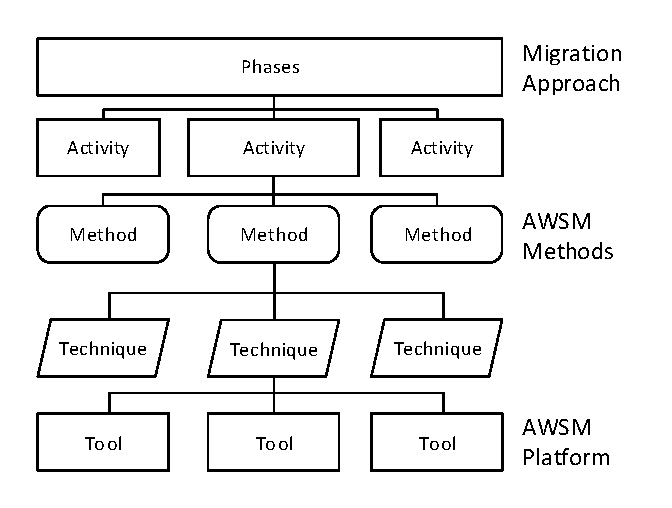
\includegraphics[width=0.99\textwidth]{../figures/remip-methods-techniques-tools.pdf}
\caption{ReMiP Taxonomy \autocite[adapted from][]{Sneed2010SoftwareMigration} mapped to AWSM}\label{fig:methods-techniques-tools}
}
\end{figure}

\hypertarget{awsm-reverse-engineering-method}{%
\subsubsection{AWSM reverse engineering method}\label{awsm-reverse-engineering-method}}

Addressing RO2, the AWSM reverse engineering method (AWSM:RE) specifies an approach to identify and manage problem and solution domain knowledge in legacy source code according to the conceptual models of legacy system and SCKM introduced before.
Unlike existing redocumentation and design recovery methods, AWSM:RE focuses on applicability for ISVs with limited resources and limited web engineering expertise.
To achieve this, AWSM:RE introduces the novel idea of \emph{crowdsourced reverse engineering} \autocite{Heil2018CSRE} and demonstrates applicability by re-formulating the problem of concept assignment \autocite{Biggerstaff1994ConceptAssignmentJournal} as classification problem that can be solved using the \emph{crowdsourcing paradigm} \autocite{Howe2006}.
Following principle P1, AWSM:RE represents reverse engineered knowledge in a queryable and interoperable way using semantic web technologies thus providing a basis for subsequent reengineering and transformation approaches.
The concretisation of the conceptual SCKM as OWL-Ontology allows adaption of AWSM:RE to different web migration methods at varying degrees of model-driven adoption, according to principle P3.
AWSM:RE is described in \cref{sec:awsm-re}.

\hypertarget{awsm-risk-management-method}{%
\subsubsection{AWSM risk management method}\label{awsm-risk-management-method}}

The AWSM risk management method (AWSM:RM) addresses RO3 by specifying a solution to demonstrate desirability and feasibility of a potential web-based version of the legacy system based on the existing software artifacts as defined in the conceptual model of the legacy system which can be achieved with only limited resources and web engineering expertise.
Unlike existing risk management methods in the early stages of web migration, it focuses on creating a concrete and tangible contribution to the business case that serves as means of communication for stakeholders to support decision making.
To achieve this, AWSM introduces the novel idea of \emph{rapid web migration prototyping} \autocite{Heil2018ReWaMP} by transferring the \emph{rapid prototyping paradigm} \autocite{Gordon1995RapidPrototyping} according to principle P4 from forward engineering into the web migration domain.
AWSM:RM defines a process for rapidly creating web migration prototypes based on the legacy system artifacts leveraging the new WebAssembly W3C standard \autocite{W3C2018WebAssembly} in compliance to principle P1.
AWSM:RM is described in \cref{sec:awsm-rm}.

\hypertarget{awsm-customer-impact-control-method}{%
\subsubsection{AWSM customer impact control method}\label{awsm-customer-impact-control-method}}

The AWSM customer impact control method (AWSM:CI) addresses RO4 by providing a mechanism to control the impact of web migration on the user bases of existing customers with limited resources and lack of web engineering expertise.
Based on the conceptual model of legacy user interfaces introduced above, AWSM:CI contributes two solutions towards this objective: it defines a visual similarity measure that allows to determine and thus control the degree of visible changes introduced into the user interface through web migration and it provides a transformation procedure creating web-based grid layouts from pixel-based legacy user interfaces based on genetic optimisation.
Unlike existing automatic analysis methods for web user interfaces that rely on DOM\footnote{Document Object Model, cf.~\autocite{W3C2015DOM}} analysis, the AWSM:CI similarity measure is applicable to both legacy and web user interfaces \autocite{Heil2016Similarity}.
To achieve this, AWSM:CI contributes to the novel field of research on visual analysis of user interfaces employing deep learning to automatically detect elements of the user interface enabling calculation of derivative measures.
Following principle P1, analysis results are made available using JSON.
AWSM:CI is described in \cref{sec:awsm-ci}.

\hypertarget{sec:remip-mapping}{%
\subsubsection{Mapping to the Reference Migration Process}\label{sec:remip-mapping}}

\cref{tbl:awsm-remip} provides a mapping of the AWSM methods onto the migration phases and disciplines of the Reference Migration Process \autocite{Sneed2010ReMiP} in order to facilitate integration with existing web migration approaches as per principle P2.
While the techniques of AWSM:RE and AWSM:RM belong to the earliest ReMiP phase, AWSM:CI techniques are conducted during Migration \& Transition.
The three methods cover several core and base disciplines each, but all are targeting the migration decision milestone as per RO1.

\hypertarget{tbl:awsm-remip}{}
\begin{longtable}[]{@{}llll@{}}
\caption{\label{tbl:awsm-remip}Mapping of AWSM Methods to ReMiP}\tabularnewline
\toprule
\begin{minipage}[b]{0.07\columnwidth}\raggedright
AWSM Method\strut
\end{minipage} & \begin{minipage}[b]{0.15\columnwidth}\raggedright
Phase\strut
\end{minipage} & \begin{minipage}[b]{0.26\columnwidth}\raggedright
Core Disciplines\strut
\end{minipage} & \begin{minipage}[b]{0.41\columnwidth}\raggedright
Base Disciplines\strut
\end{minipage}\tabularnewline
\midrule
\endfirsthead
\toprule
\begin{minipage}[b]{0.07\columnwidth}\raggedright
AWSM Method\strut
\end{minipage} & \begin{minipage}[b]{0.15\columnwidth}\raggedright
Phase\strut
\end{minipage} & \begin{minipage}[b]{0.26\columnwidth}\raggedright
Core Disciplines\strut
\end{minipage} & \begin{minipage}[b]{0.41\columnwidth}\raggedright
Base Disciplines\strut
\end{minipage}\tabularnewline
\midrule
\endhead
\begin{minipage}[t]{0.07\columnwidth}\raggedright
AWSM:RE\strut
\end{minipage} & \begin{minipage}[t]{0.15\columnwidth}\raggedright
Preliminary Study\strut
\end{minipage} & \begin{minipage}[t]{0.26\columnwidth}\raggedright
Legacy Analysis, Requirements Analysis\strut
\end{minipage} & \begin{minipage}[t]{0.41\columnwidth}\raggedright
Configuration \& Change Management, Project Management, Migration Environment\strut
\end{minipage}\tabularnewline
\begin{minipage}[t]{0.07\columnwidth}\raggedright
AWSM:RM\strut
\end{minipage} & \begin{minipage}[t]{0.15\columnwidth}\raggedright
Preliminary Study\strut
\end{minipage} & \begin{minipage}[t]{0.26\columnwidth}\raggedright
Requirements Analysis, Target Design\strut
\end{minipage} & \begin{minipage}[t]{0.41\columnwidth}\raggedright
Project Management, Staff Qualification\strut
\end{minipage}\tabularnewline
\begin{minipage}[t]{0.07\columnwidth}\raggedright
AWSM:CI\strut
\end{minipage} & \begin{minipage}[t]{0.15\columnwidth}\raggedright
Migration \& Transition\strut
\end{minipage} & \begin{minipage}[t]{0.26\columnwidth}\raggedright
Target Design, Implementation\strut
\end{minipage} & \begin{minipage}[t]{0.41\columnwidth}\raggedright
Migration Environment\strut
\end{minipage}\tabularnewline
\bottomrule
\end{longtable}

\hypertarget{sec:platform}{%
\section{AWSM Platform}\label{sec:platform}}

The AWSM Platform comprises all support tools for the AWSM methodology.
It is a web-based reverse engineering and web migration management platform to support management and migration engineer stakeholders (cf.~\cref{tbl:stakeholders}), providing a migration monitoring and management dashboard with software quality visualisations, a legacy knowledge repository with a query endpoint, a concept-assignment-based reverse engineering tool, knowledge discovery tools, a process guidance and generation tool for rapid web migration prototyping and a customer impact control and web-ui generation tool.
To achieve good integration into ongoing development activities (cf.~C4 Agile), the AWSM Platform integrates with software project management platforms for management stakeholders and with integrated development environments (IDEs) for migration engineer stakeholders (similar to ARTIST Methodology Process Tool (MPT)
{[}\textcite{ARTIST2015ProcessFramework};\textcite{Menychtas2014ARTISTJournal}{]}).
Principle P1 drives the design of the AWSM Platform.
The tools which constitute the AWSM Platform addressing research objectives RO2, RO3 and RO4 are described in the following chapters together with the AWSM methods which they support.
The AWSM Strategy Selection Decision Support System, which addresses RO1, is described in the following section.

\hypertarget{sec:s2dcs}{%
\subsection{AWSM Strategy Selection Decision Support System}\label{sec:s2dcs}}

The AWSM Strategy Selection Decision Support System (S2DCS) is a part of the AWSM Platform that supports ISVs to select a global web migration strategy (cf.~ReMiP \emph{strategy selection} discipline \autocite{Sneed2010ReMiP,Gipp2007ReMiP}).
According to principle P2, AWSM is a methodology that provides solutions addressing the identified gaps in current web migration approaches, designed to be open for integration with existing web migration reengineering and transformation process models.
As shown in \cref{sec:approaches}, there is a wide range of approaches.
In our systematic mapping study \autocite{Heil2017Survey}, we identified and evaluated 122 primary studies, comprising not only academic publications, but also existing software tools.
Selecting a suitable approach for the specific situation among this plethora of possibilities is difficult for ISVs.

Thus, based on the results of the survey \autocite{Heil2017Survey}, a decision support system was created.
Addressing RO1, the S2DCS supports ISVs to commence a web migration by enabling them to select a suitable strategy based on existing approaches and tools.
Using S2DCS ISVs can either decide to employ the approach that suits best to their specific web migration problem, or build their own composite strategy based on the information provided from a set of appropriate approaches.
As S2DCS represents a \emph{faceted search} interface \autocite{Tunkelang2009FacetedSearch} to a knowledgebase of existing approaches and tools, ISVs with limited resources and lack of web migration expertise are supported in formation of their migration strategy by being given easy access to a wide range of information that would have otherwise required extensive time, effort and expertise to accumulate.

Supporting non-technical Management stakeholders as described in \cref{sec:problem-analysis-results}, the faceted search is realised as a guided dialogue interaction.
The S2DCS user answers a set of questions dynamically created from the available criteria and values in order to specify his web migration scenario, i.e.~the as-is and to-be state \autocite{Nguyen2009} and constraints.
The answers form the search facets that define the query on the knowledgebase.
To construct the result set, candidate approaches are ranked according to the compliance factor formalism introduced in \cref{sec:compliance-ranking} and ordered by their rank.
The criteria for selecting approaches are defined by target and source system characteristics (e.g.~architectures, technologies), supported migration phases (e.g.~legacy analysis, implementation etc.
cf.~ReMiP) and dynamic criteria depending on selection of the other criteria (e.g.~SOAP or REST when SOA target was selected).

The user can review the details of the resulting approaches and access information about authors, year of creation, a brief description, the main project or publication URL, complimentary linked resources such as reports and case studies, as well as available evidence of successful application, industrial relevance and tool support.
The S2DCS is designed to allow the selection criteria, catalogue data and the dataset of the knowledgebase to be extended through configuration to allow updating the web migration approaches.
In the context of AWSM, S2DCS supports ISVs to determine a suitable web migration strategy (cf.~principles P2 and P3) into which the AWSM methodology gets embedded to address the identified shortcomings of existing approaches.

\todo{TODO:screenshot}-in-appendix, URL ref
